\chapter{密度泛函理论基础} \label{chap:dft}

二十世纪二十年代,Thomas-Fermi{建议的自由电子模型}\cite{PCPS23-542_1927,ZP48-73_1928}中,将经典体系的总能表示成为电子密度$\rho$的函数\cite{Parr-Yang,CR91-651_1991},可以看成密度泛函(Density Functional)思想的源头;五十年代Slater用局域电荷密度代替离域的波函数乘积,简化了Hartree-Fock方法\cite{MPCPS24-111_1928,ZP61-126_1930, PR32-339_1928}中交换能的计算,这就是著名的X\,$\alpha$方法\cite{PR81-385_1951},该方法表明,考虑量子效应后,电子体系的能量仍可以用电子密度近似表示
。%这些研究都显示,体系的能量有可能表示成为基态密度的函数。 %最早}) {思想的源头}可以上溯到%理论})
采用电子密度计算体系总能量,最大的优点是有效地减少变量的数目,极大地方便了应用理论方法研究电子体系,由此带动了密度泛函表示体系性质的研究热潮。但是真正将
密度泛函理论\textrm{(Density Functional Theory,~DFT)}确立为严格的理论,要等到六十年代,Hohenberg和Kohn%最基本的变量是体系单粒子})
完成密度泛函理论的基本定理的证明\cite{PR136-B864_1964}。
Hohenberg-Kohn定理表明,体系的基态性质(如总能量)完全由%单})
%粒})
基态{电}子密度决定;随后,Kohn和Sham\cite{PR140-A1133_1965}%采用了与相互作用体系有相同单粒子密度的无相互作用体系的动能近似来近似计算相互作用体系的动能,把剩余部分都放在交换-相关能项中予以考虑。本质上,这个方法把单粒子波函数又引入了密度泛函理论,但是基本解决了动能计算的问题。在他们的工作基础上,各种近似的交换-相关能泛函形式\cite{CJP58-1200_1980,PRB45-13244_1992,PRA38-3098_1988,PRB33-8822_1986,PRB37-785_1988}被提出来并})
{提出了用基态密度表示体系总能量的成近似方案,使密度泛函理论可应用于实际体系的量子力学计算。七十年代之后,密度泛函理论的研究主要集中在寻求更精确的能量密度泛函表达形式上,其中有些泛函已被}广泛应用于%计算各类})
原子、分子和固体体系{的计算中\cite{CJP58-1200_1980,PRB45-13244_1992,PRA38-3098_1988,PRB33-8822_1986,PRB37-785_1988}}。

\section{Hohenberg-Kohn定理}
Hohenberg-Kohn定理\cite{PR136-B864_1964}包含两部分{内容}:
\begin{itemize}
	\item 第一部分指出,多%粒})
{电}子体系的外势由其%基态性质与
基态%单})
%粒})
{电}子密度%之间存在一一对应关系,这部分是密度泛函理论的基础
决定(除可能相差一个常数以外),从而体系的基态波函数以及所有其它性质均由其基态电子密度决定
;\item 第二部分指出体系基态总能量{泛函}在体系基态%单})
%粒})
{电}子密度处取极小{值},这部分%给出})
{提供}了从%单}) %粒})
{电}子密度计算体系基态能量的基本方法。
\end{itemize}
%Hohenberg-Kohn
简单证明如下:

%设})
N个粒子相互作用量子力学体系的%Hamiltonian})
{基态总能量}可表示为:
\begin{equation}
	{E_{\mathrm{gs}}[\Psi]}%F_{\mathrm{HK}}[\rho]})
=\langle\Psi%[\rho]})
|\hat{T}+\hat{V}+\hat{W}|\Psi%[\rho]})
\rangle
	\label{eq:DFT_01}
\end{equation}
其中$\hat{T}$是动能算符,$\hat{V}$是外势%、即通常的局域单粒子势})
,$\hat{W}$为%粒})
{电}子间相互作用势{,$|\Psi\rangle$是基态波函数}。假设两个体系的外势分别为$\hat{V}$和$\hat V^{\prime}$,它们之间相差不为常数,这两个体系的非简并基态分别为$|\Psi\rangle$和$|\Psi^{\prime}\rangle$,其基态的本征方程分别为:
$${\hat H\Psi=}\bigl(\hat{T}+\hat{V}+\hat{W}\bigr)|\Psi\rangle=E_{\mathrm{gs}}|\Psi\rangle$$
$${\hat H^{\prime}\Psi=}\bigl(\hat{T}+\hat V^{\prime}+\hat{W}\bigr)|\Psi^{\prime}\rangle=E_{\mathrm{gs}^{\prime}}|\Psi^{\prime}\rangle$$

%假设})
{根据量子力学原理,}$|\Psi\rangle{\neq}|\Psi^{\prime}\rangle$,%则上两式相减可得}):
% $$%\big(\hat{V}-\hat V^{\prime}\big)|\Psi\rangle=\big(E_{gs}-E^{\prime}_{gs}\big)|\Psi\rangle}) $$
%因为$\hat{V}$和$\hat V^{\prime}$是乘积算符,从上式可知,$\big(\hat{V}-\hat V^{\prime}\big)=\big(E_{gs}-E^{\prime}_{gs}\big)=\text{const}$,这与$\hat{V}$和$\hat V^{\prime}$之间相差不为常数矛盾,因此$\hat{V}$和$|\Psi\rangle$之间存在一一对应关系。})
由变分原理可知:
$$E_{\mathrm{gs}}=\langle\Psi|\hat{H}|\Psi\rangle<\langle\Psi^{\prime}|\hat{H}|\Psi^{\prime}\rangle$$

设$|\Psi\rangle$和$|\Psi^{\prime}\rangle$对应的%单})
%粒})
{电}子密度分别为$\rho(\vec{r})
$和$\rho^{\prime}(\vec{r})$,{$v(\vec r)$为单个电子受到的外势的作用能,则}有
$$\langle\Psi^{\prime}|\hat{H}|\Psi^{\prime}\rangle=\langle\Psi^{\prime}|\hat H^{\prime}+\hat{V}-\hat V^{\prime}|\Psi^{\prime}\rangle=E^{\prime}_{gs}+\int{\rho^{\prime}(\vec{r})[v(\vec{r})-v^{\prime}(\vec{r})]\textrm{d}^3\vec{r}}$$
%相应的,从$E^{^{\prime}}_{gs}$出发})
{类似地}可以得到不等式
$$E^{^{\prime}}_{gs}<E_{gs}+\int{\rho(\vec{r})[v^{\prime}(\vec{r})-v(\vec{r})]\textrm{d}^{3}\vec{r}}$$

%假设})
{如果}$\rho(\vec{r})\!=\!\rho^{\prime}(\vec{r})$,把上面两个不等式相加可以得到$E_{gs}+E^{\prime}_{gs}\!<\!E_{gs}+E^{\prime}_{gs}$,这显然%与假设矛盾,因此$\rho(\vec{r})$与v可以表示的基态$|\Psi\rangle$之间有一一对应关系})
{不能成立。亦即不可能出现不同的外势产生相同的电子密度的情况}。由此可以得出结论,体系的基态%单})
%粒})
{电}子密度和体系的外势(除了相差一个常数之外)一一对应%,})
{。}%也就是说,})
{因为$\rho(\vec r)$唯一地确定体系中电子的数目$N$,故}体系%的一切})
{%基态
的\textrm{Hamiltonian}、从而全部}性质都%可以})
由体系的基态%单})
%粒})
{电}子密度完全决定。{特殊地,体系基态总能量是它的基态电子密度的泛函,记作$E[\rho]$。
	
设有一电子密度$\tilde\rho(\vec r)$,满足约束条件
\begin{displaymath}
	\begin{aligned}
		\tilde\rho(\vec r)\!&\geqslant\!0\\
		\int\tilde\rho(\vec r)\textrm{d}^3\vec r&\!=\!N
	\end{aligned}
\end{displaymath}
$\tilde\rho(\vec r)$来自某个\textit{v}\,-\,可表示的基态波函数$\tilde\Psi$(称为\textit{v}\,-\,可表示的电子密度)。设与体系基态波函数$\Psi$对应的电子密度为$\rho_0(\vec r)$,若$\tilde\rho(\vec r)\!\neq\!\rho_0(\vec r)$,则根据上面的讨论可知,$\tilde\Psi\!\neq\!\Psi$,$E[\tilde\rho]$\,$\geqslant$\,$E[\rho_0]$。}

%从上面的结论我们可以定义作为单粒子密度$\rho(\vec{r}) $泛函的体系基态能量的形式。设一$N$个粒子体系的外势场为$\hat{V_{0}}$,})
{设}与$\rho(\vec{r})$%一一})
对应的%某一N个粒子})
体系波函数为$|\Psi[\rho]\rangle$,%定义该})
体系的基态总能量作为$\rho(\vec{r})
$的泛函%形式})
{可表达}为:
\begin{equation}
	E[\rho]=\langle\Psi[\rho]|\hat{T}+\hat{V}+\hat{W}|\Psi[\rho]\rangle
	\label{eq:DFT_02}
\end{equation}
%由变分原理可知,体系本身的基态单粒子密度使得$E_{v_{0}}[\rho]$取极小,因此可以通过寻找能量泛函的极小值点来确定体系的基态能量和基态粒子密度}
{因为由外势产生的势能是电子密度$\rho(\vec r)$的简单泛函,}体系的{基态}总能量泛函可以写成:
\begin{equation}
	E[\rho]=F_{\mathrm{HK}}[\rho]+\int\rho(\vec{r})v(\vec{r})\textrm{d}^3\vec{r}
	\label{eq:DFT_03}
\end{equation}
其中$F_{\mathrm{HK}}[\rho]=\underset{\Psi\to\rho}{\mathrm{Min}}\langle\Psi[\rho]|\hat{T}+\hat{W}|\Psi[\rho]\rangle$%。})
{,}%从上式可以看出,$F_{\mathrm{HK}}$的形式}
与%$v_{0}$})
{$v(\vec r)$}没有关系,%只与动能和离子间相互作用能的形式有关。对于我们最通常研究的原子、分子和固体体系而言,$F_{\mathrm{HK}}$的形式都是一致的。但是})
{是一个普适的能量泛函。}

到目前为止,$F_{\mathrm{HK}}$的%具体})
{精确表达形}
式还没有得到,%一般都采用近似的方法})
{只能作近似处理}。Thosmas-Fermi%理论})
{模型}%实际上就是一个对$F_{\mathrm{HK}}$近似的理论,但是由于动能泛函的误差很})
{可以看作是对$F_{\mathrm{HK}}[\rho]$泛函采取粗略近似的密度泛函理论。由于误差太}大,Thomas-Fermi%理论})
{模型}既不能%得到})
{说明}原子体系%正确的})
电子密度的壳层结构,也不能%得到})
{说明存在}稳定%的})
分子{的事实}。%后来经过})
Dirac\cite{PCPS26-376_1930}和Weizsacker\cite{ZP96-431_1935}对能量泛函的改进取得%了})
一定%的进展})
{成功},但%是同实验结果相比,仍然有比较大的差距})
{没有取得实质性的进展}。

上述%的证明})
只讨论了非简并基态的问题{。}Kohn证明\cite{Bassani-Fumi-Tosi},对于%简并体系基态})
{体系简并基态}的情况,虽然%单})
%粒})
{电}子密度和体系的基态波函数之间的一一对应关系不再成立,但是同样可以定义一个普适的能量泛函$F_{\mathrm{HK}}$,体系的基态%单})
%粒})
{电}子密度使%得})
体系%的})
基态{总}能量{泛函}取极小{值的定理}仍然成立。%前})
{在上}面的证明%隐含的一个})
{中}假设%是我们所取的})
%单})
%粒})
{电}子密度$\rho$是\textit{v}\,-\,可表示的,%即$\rho$是由某个外势决定的Hamiltonian算符的基态单粒电子密度})
{这使得通过变分方法寻找能量泛函的极小值难于实现}。Levy\cite{PNAS76-6062_1979}证明,实际上,只要$\rho$是
%\it v}-})
{$N$}可表示的,即$\rho$%是与})
{来自}某个$N$电子体系的基态波函数%相对应})
,上面的定理也%能够})
成立。可以证明\cite{PRB12-2111_1975,IJQC24-243_1983},任意一个合理的%单})
%粒})
{电}子密度都是%{\it v}-}
{$N$}可表示的,这样就%可以})
基本解决{了}变分空间的%选取})
问题。

\section{Kohn-Sham方程}
%对于})
{根据}Hohenberg-Kohn定理,只要%得到})
{知道}体系的总能量的{密度}泛函形式,就可以通过对%单})
%粒})
{电}子密度%作})
变分求得体系的基态%单粒})
{总能量和基态的电}子密度%和基态能量})
。与%通常的})
对波函数%作})
变分求%得})
体系基态%性质})
{总能量}的方法相比,波函数是3N%-维})
{维空间中的}函数,而%单})
%粒})
{电}子密度只是三维{空间中的}函数,因此这种方法有%巨})
{很}大的优越性。但是%由于很难})
{迄今无法}得到%比较})
精确的能量密度
泛函形式,特别是体系的动能密度
泛函的精确%度对计算体系性质有很大的影响})
{形式。为避开这一困难},Kohn和Sham\cite{PR140-A1133_1965}提出%了用具有与相互作用体系单粒电子密度相同但无相互作用体系的动能来近似计算相互作用体系动能的方法,这种})
{以下}方法%比较好地})
解决%了})
动能泛函的计算问题。%他们的})
具体%计算})
方法如下:假设存在一个外势为$v_s$的无相互作用多%粒})
{电}子体系,其基态%单})
%粒})
{电}子密度$\rho$与%我们所})
{要}研究的一个多电子相互作用体系的基态%单})
%粒})
{电}子密度相同。这个无相互作用体系的%单})
%粒})
{电}子密度为:
$$\rho(\vec{r})=\sum_{i=1}^{N}\langle\varphi_{i}|\vec{r}\rangle\langle\vec{r}|\varphi_{i}\rangle$$
其中$\varphi_i(i\!=\!1,\cdots,N)$是该体系能量最低的$N$个{单电子}本征态。该体系的动能为:\linebreak $T_{s}[\rho]\!=\!\sum\limits_{i=1}^{N}\langle\varphi_{i}|\hat{T}|\varphi_{i}\rangle$。
用这个无相互作用体系的动能作为%我们})
{要}研究的相互作用体系的动能近似{值},可以把相互作用体系的%动能})
{基态能量密度泛函}写成如下形式:
\begin{equation}
  \label{eq:dft-1}
E[\rho]=T_{s}[\rho]+\int{v(\vec{r})\rho(\vec{r})\textrm{d}^3\vec{r}}+\frac 12\iint{\rho(\vec{r})w(\vec{r},\vec r\,^{\prime})\rho(\vec r\,^{\prime})\textrm{d}^3\vec{r}\textrm{d}^3\vec r\,^{\prime}}+E_{XC}[\rho]
\end{equation}
其中{$w(\vec r, \vec r\,^{\prime})$为两个电子间的相互作用能。}交换-相关能泛函的形式为:

\begin{equation} 
  \label{eq:dft-2}
  E_{XC}[\rho]=F_{\mathrm{HK}}[\rho]-\frac 12\iint{\rho(\vec{r}) w(\vec{r},\vec r\,^{\prime})\rho(\vec r\,^{\prime})\textrm{d}^3\vec{r}\textrm{d}^3\vec r\,^{\prime}}-T_{s}[\rho]
\end{equation}
利用$T_s$和$\rho$的表达式,%对})
{由}总能量%作})
{在$\{\varphi_i, i\!=\!1,\cdots, N\}$满足正交归一条件下对$\{\varphi_i\}$}变分,即%可以})
得到Kohn-Sham方程:
\begin{equation} \label{eq:dft-3}
	\bigl(\hat{T}+\hat{V}_{\mathrm{eff}}\bigr)|\varphi_{i}\rangle=\varepsilon_{i}|\varphi_{i}\rangle{,\quad i=1,\cdots,N,\cdots}
\end{equation}
其中
\begin{equation} \label{eq:dft-4}
	V_{\mathrm{eff}}(\vec{r})={v}(\vec{r})+\int{w(\vec{r},\vec r\,^{\prime})\rho(\vec r\,^{\prime})\textrm{d}^3{\vec r\,^{\prime}}+\frac{\delta E_{XC}}{\delta\rho(\vec{r})
}}
\end{equation}
式\eqref{eq:dft-4}右边第一项%中})
${v}(\vec{r})
$为外势,第二项为%粒})
{电}子间经典的{Coulomb}相互作用势,第三项是交换-相关势。%对于我们所关心的原子、分子和固体等多电子体系而言,\eqref{eq:dft-4}式中的外势为核吸引势,粒子间经典相互作用势是电子间的Coulomb势。})

以上推导中假设任意一个相互作用%的{\it v}-可表示的单粒})
{体系的基态电}子密度%也是})
{都有一个}与之有相同基态电子密度的无相互作用%的{\it v}-可表示单粒})
{的体系相对应}。可以证明,按照该方法构造的无相互作用体系基态如果是非简并的,即这个无相互作用体系的基态可以用单行列式波函数表示,则用这个单行列式波函数构造的%单粒})
{基态电}子密度与相互作用体系的%单粒})
{基态电}子密度是一致的%,但是如果无相互作用体系的基态是简并的,相互作用{\it v}-可表示单粒子密度是否仍然与由单行列式波函数构造的无相互作用体系单粒子密度对应的问题还没有得到解决})
。\cite{PNAS76-6062_1979,IJQC24-243_1983}

对于{电子}自旋{密度}%极化的情况,从})
{不恒为零的体系,推广}Hohenberg-Kohn定理%可以知道,体系基态自旋为})
{的推导过程和近似处理方法,可以得到对于体系的}$\alpha$%})
自旋和%为$\beta$的})
{$\beta$自旋}电子的{\textrm{Kohn-Sham}方程,被称为自旋密度泛函理论\textrm{(SDFT)}。}%密度从原理上可以由体系总电子密度完全决定;但是如果要研究})
{在}研究一些体系的磁学性质或者处于解离极限的分子的性质{时},%在现有泛函基础上,只有})
采用%把自旋$\alpha$和自旋$\beta$的电子分开处理的})
自旋密度泛函方法才能得到合理的结果{。}%而且})
对于开壳层体系%而言})
,用自旋密度泛函方法%的结果})
通常比不{区}分自旋的密度泛函方法结果要好。%自旋密度泛函理论的基本原理和Kohn-Sham方程很容易用类似的推导方法得到,在此不作推导了。})

Kohn-Sham方程的%这个})
实质,是把动能泛函的主要部分分离出来,将剩余%不太重要的动能})
部分放到交换-相关能中。由于该方程%基本})
{比较好地}解决了%计算})
动能泛函的{计算}问题,%这个方法})
使得密度泛函方法能够比较精确地研究电子体系的性质。有必要指出,Kohn-Sham方程虽然把单%粒})
%{\kaishu 电}
电子波函数引进密度泛函理论,但它是{\heiti 形式上的单粒子方程},%从理论上讲只利用单Slater行列式就})
因为方程中包括泛函的形式表示的交换-相关作用%计算})
,这是对电子间的多体关联的一种近似考虑,%而传统的量子化学方法如果要考虑电子之间的相关能效应,则必须采用多Slater行列式的方法,Kohn-Sham方程})
{相比}传统的量子%化})
{力}学方法,密度泛函方法有明显的%})
优越%性})
{之处},基于Kohn-Sham方程的密度泛函方法也成为电子尺度计算最重要的{理论}方法之一。

\section{交换-相关能泛函}
Kohn-Sham方程%从})
理论上%讲})
是%一个})
严格的方程,但是要把它用于具体计算,就需要%解决})
{知道}交换-相关能泛函的具体形式。%从上一节的推导可以看出,})
Kohn-Sham%理论})
提出的交换-相关能的含义与从头计算方法的交换和相关能的含义有%很})
{较}大的差别{。现有}密度泛函理论中,习惯上将交换能定义为用Kohn-Sham轨道按照Hartree-Fock交换能%形})
{表达}式计算得到的能量,相关能则包含两部分,一部分是相互作用体系动能和对应的无相互作用体系动能{之}差,另一部分是相互作用体系中粒子间的相互作用能与经典相互作用{能}和交换能%的})
{之}差。密度泛函{理论}中的交换-相关能泛函的精确形式还%没有})
{无法}得到,只能通过{考虑}一些{应满足的}具体%的})
物理%考虑})
{条件}和合理的假设得到近似的交换-相关能泛函。最简单的近似就是由Kohn和Sham提出的局域密度近似%方法})
{泛函}(local density approxmiation, LDA)\cite{PR140-A1133_1965}{。}局域密度近似基于均匀电子气模型得到的,直觉上,应该主要对于电子密度变化缓慢的体系{才会}是%个})
比较好的近似,而实际上对于原子、分子和某些价电子密度%变化})
剧烈变化的固体,局域密度近似方法仍然能够得到比较合理的结果。不过,为了进一步提高密度泛函方法对原子、分子以及扩展体系的计算精度,应该需要考虑%到})
电子密度的不均匀性。通过引入电子密度的梯度对{局域近似的}交换-相关能的{泛函}形式加以校正,%即所谓的})
{就是}梯度展开近似(Gradient Expansion Approximation, GEA)%和})
{或}一般梯度近似(Generalized Gradient Approximation, GGA),%即})
此时能量泛函不仅依赖于局域密度值的分布,还与密度梯度有关,这在一定程度上改善LDA的计算结果。比较重要的GGA交换能泛函有P86$_x$\cite{PRB33-8800_1986}、B88\cite{PRA38-3098_1988}、PW91\cite{PRB46-6671_1992,PRB48-4978_1993,PRB54-16533_1996,PRB57-14999_1998}、PBE\cite{PRL77-1396_1996,IBID78-1396_1997}、HCTH\cite{JCP109-6264_1998}等。

由于在交换-相关能泛函的定义中包含了一部分动能的贡献,因此很多研究者考虑{到}在交换-相关{能}泛函中应该包括动能密度为变量,%这就是所谓的})
{提出}\textit{meta}-GGA泛函。自1980年代末以来,比较有代表性的\textit{meta}-GGA交换能泛函有BR89\cite{PRA39-3761_1989}、\linebreak VSXC\cite{JCP109-400_1998}、tauPBE\cite{JCP111-911_1999}、PKZB\cite{PRL82-2544_1999,PRL82-5179_1999}、B00\cite{JCP112-4020_2000}、PCS00\cite{JCP113-10013_2000}等。

为了提高各种近似{能量}泛函的%计算结果的})
精度,从1990年代初起,基于绝热关联%(下面会详述)})
{的推理},Becke提出把部分按Hartree-Fock方法计算的交换能加入到能量密度泛函中的思想{,}%从而})
构造出了一系列%的所谓})
杂化型%的})
交换-相关{能}泛函,其中比较重要的是“半对半(half and half)”泛函\cite{JCP98-1372_1993}、B3P\cite{JCP98-5648_1993}、B3LYP\cite{JPC98-11623_1994}、B1B95\cite{JCP104-1040_1995}等。

由于%对})
相关能的物理%定})
{含}义不%很})
{够}清晰,而且相关能的数值比交换能小一个数量级,既比较难准确估计,又不是计算中误差的最主要来源,因此提出的{近似}相关能泛函%模型})
比交换能泛函%模型})
少一些。最早提出把相关能表示成电子密度泛函的是Wigner\cite{PR46-1002_1934},他的公式适用于均匀电子气:
\begin{equation}
  E_C=-\dfrac a{r_s+b}
  \label{eq:dft-16}
\end{equation}
其中$a$、$b$是参数,$r_s$\,=\,$\left(\dfrac3{4\pi\rho}\right)^{\frac13}$称为表观半径。%实际上})
对%于})
均匀电子气的相关能并没有统一\linebreak 的解析式。von Barth\cite{JPC5-1629_1972}和Gunnarsson\cite{PRB13-4274_1976}等人都提出过一些近似的式子。1980年,\linebreak Vosko、Wilk和Nusair\cite{CJP58-1200_1980}利用Ceperley和Alder\cite{PRL45-566_1980}用量子Monte Carlo方法计算得到的{均匀电子气}相关能数据拟合出一个%均匀电子气的})
相关能的%公})
{表达}式,即最常用的VWN%公})
{表达}式。后来Perdew和Wang\cite{PRB45-13244_1992}把他们的%公})
{表达}式简化并重新拟合了参数。

以上相关能%公式})
{泛函}都是针对均匀电子气的,比较常用的考虑了梯度校正的相关能泛函%公})
{表达}式有P86$_c$\cite{PRB33-8822_1986}、LYP\cite{PRB37-785_1988}、Bc88\cite{JCP88-1053_1988}、PW91\cite{PRB46-6671_1992,PRB48-4978_1993,PRB54-16533_1996,PRB57-14999_1998}等。

按照Perdew的建议\cite{Perdew-Schmidt_2001},现有的交换-相关能密度泛函可以分为以下几类:
\begin{enumerate}
  \item LDA: 即泛函只与密度分布的局域值有关;
  \item GGA: 泛函所依赖的变量除了局域密度之外,还包括局域密度的梯度;
  \item \textit{meta}-GGA: 泛函依赖的变量还包括动能密度;
  \item {杂化(hybrid)泛函}: 泛函与占据轨道有关;
  \item 完全非局域泛函: 泛函与所有的占据和非占据轨道都有关,属于理想泛函但不%现实})
{切合实际}。
\end{enumerate}
\begin{figure}[!h]
\centering
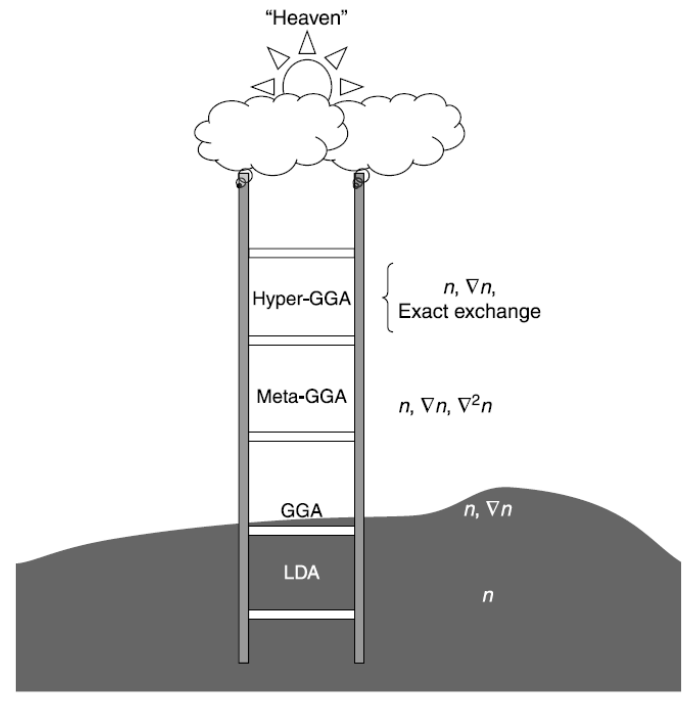
\includegraphics[height=3.4in,width=3.18in,viewport=10 5 680 700,clip]{Jacobi-ladder.png}
\caption{\small The schematic digram of Jacob's Ladder for DFT.\cite{Perdew-Schmidt_2001,Science298-759_2002}}
\label{Fig:Jacob-Ladder}
\end{figure}

上述{各类}泛函%的类别})
从上到下越来越接近%化学})
精确值,因此被形象地视为``Jacob's Ladder''(登天梯,见图\ref{Fig:Jacob-Ladder}):~将\textrm{LDA~}视为第一级阶梯,\textrm{GGA~}视为第二级阶梯,更复杂的泛函形式视为第三级及更高的阶梯。\cite{PRL91-146401_2003}但在密度泛函中过度引入轨道将会%造成})
{大大增加}计算量%的大大增加})
,失去密度泛函理论对%一般})
从头计算方法的优势,因此是{并}不可取的。
下面对每一类中最重要的泛函作一些简单的介绍。

\subsection{局域密度近似和LDA泛函}
局域密度近似是Kohn和Sham提出的最简单的一种近似处理交换-相关能的方法。交换-相关能{泛函}的具体形式取为:
\begin{equation}
  \label{eq:dft-5}
  E_{XC}^{\mathrm{LDA}}[\rho]=E_X^{\mathrm{LDA}}[\rho]+E_C^{\mathrm{LDA}}[\rho]=\int\varepsilon_X[\rho]\rho(\vec{r}) \textrm{d}^3\vec{r}+\int\varepsilon_C[\rho]\rho(\vec{r}) \textrm{d}^3\vec{r}
\end{equation}
其中$\varepsilon_X[\rho]$和$\varepsilon_C[\rho]$分别为{一个电子的}交换能和相关能%密度})
。上式表明空间每一个点的交换能密度和相关能密度只是取决于该点的电子密度,而与其他点的电子密度无关。对{于均匀电子气,}$\varepsilon_X[\rho]$和$\varepsilon_C[\rho]$%的选取可按照均匀电子气中交换-相关能和电子密度的关系得到,})
{为常数%,等于体系的总电子交换能(或相关能)除以体系的体积和电子密度
。}对于非均匀电子气%而言})
,%这样选取的$e_X(\rho)$和$e_C(\rho)$的物理图象相当于})
{可以设想}把空间分割为无穷多个%非常})
{无限}小的区域,%假设})
{可以认为}电子的密度在每个小的区域内都是均匀的,每个小区域中的交换-相关能都%采用})
{可以按}均匀电子气%模型下})
的交换-相关能{计算},整个体系的交换-相关能就可以写成\eqref{eq:dft-5}式的形式。{采用}这种模型{,}%下的})
\textrm{Kohn-Sham~}方程的交换势表达为:
\begin{equation} \label{eq:dft-6}
	V_X^{\mathrm{LDA}}(\vec{r}) =\dfrac {\delta E_X^{\mathrm{LDA}}}{\delta\rho(\vec{r}) }=-\dfrac 32\alpha\left\{\dfrac3\pi\rho(\vec{r}) \right\}^{1/3}
\end{equation}
Kohn和Sham等从总交换能的角度出发%给})
{得}出$\alpha=2/3$\cite{PR140-A1133_1965},Slater从交换势的角度出发,%给})
{得}出$\alpha=1$\cite{PR81-385_1951},对原子、分子体系的计算表明,选取$\alpha$约为0.7\cite{AQC6-1_1972,Slater-4_1974}结果更好。

对于用自旋密度泛函方法处理的自旋极化体系%的情况})
,%此时的})
交换能{泛函的}形式可以写成\cite{PRA20-397_1979}
\begin{equation} \label{eq:dft-7}
E_X[\rho_{\alpha},\rho_{\beta}]=\frac12E_X^{0}[2\rho_{\alpha}]+\frac12E_X^{0}[2\rho_{\beta}]
\end{equation}
其中$E_X^{0}[\rho]=E_X\bigl[\dfrac 12\rho_{\alpha},\dfrac 12\rho_{\beta}\bigr]$

相关能包含相同自旋电子间的相互作用和不同自旋电子间相互作用,不可能把相关能泛函也分解成为两种自旋电子的相关能的贡献和。一般采用Stoll\cite{TCA49-143_1978}的定义,将局域密度近似的相关能泛函写成如下形式:
\begin{equation}
  E_C=E_C^{\alpha\beta}+E_C^{\alpha\alpha}+E_C^{\beta\beta}
  \label{eq:dft-17}
\end{equation}

把局域密度近似引入自旋密度泛函理论就是通常所说的局域{自旋}密度近似(local spin-density approximation, LSDA),LSDA中的交换能{泛函}%形})
{表达}式可以%结合})
{由}\eqref{eq:dft-7}式和\eqref{eq:dft-6}式%给})
{得}出{。}相关能泛函的形式可以写成:
$$E_C^{\mathrm{LSDA}}[\rho_{\alpha},\rho_{\beta}]=\int{\varepsilon_C(\rho,\varsigma)\rho\,\textrm{d}^3\vec{r}}$$
其中$\varsigma=(\rho_{\alpha}-\rho_{\beta})
/(\rho_{\alpha}+\rho_{\beta})
$,$\rho_{\alpha}$和$\rho_{\beta}$分别是自旋为$\alpha$和自旋为$\beta$的电子密度。均匀电子气相关能的解析形式很难求得,但是可以用数值方法计算得到%其})
数值结果,Vosko等\cite{CJP58-1200_1980}用解析式拟合%出})
精确的数值计算结果,得到局域密度近似下的相关能泛函VWN表达式{。}%但是})
他们给出的表达式%太})
{比较}复杂,Perdew和Wang\cite{PRB45-13244_1992}%又})
把它改%写})
成%为})
{比较}简单的形式,得到%的})
{一个电子的}相关能%密度})
{的}表达式为:
\begin{equation}
  \label{eq:dft-8}
  \varepsilon_C^{\mathrm{LDA}}(r_s,\varsigma)=\varepsilon_C^{\mathrm{LDA}}(r_s,0)+a_C(r_s)\dfrac{f(\varsigma)}{f^{\prime\prime}(\varsigma)}(1-\varsigma^4)+[\varepsilon_C(r_s,1)-\varepsilon_C(r_s,0)]f(\varsigma)\varsigma^4
\end{equation}
其中$r_s=\left[\dfrac 3{4\pi}\bigl(\rho_{\alpha}+\rho_{\beta}\bigr)\right]^{-1/3}$,$f(\varsigma)=[(1+\varsigma)^{4/3}+(1-\varsigma)^{4/3}-2]/(2^{4/3}-2)$,\\$\varepsilon_C(r_s,0)$,$\varepsilon_C(r_s,1)$和$-a_C(r_s)$由经验公式
$$G(r_s,A,\alpha_1,\beta_1,\beta_2,\beta_3,\beta_4,p)=-2A(1+\alpha_1r_s)\ln\left[1+\dfrac1{2A(\beta_1r_s^{1/2}+\beta_2r_s+\beta_3r_s^{3/2}+\beta_4r_s^{p+1})}\right]$$
计算{,}其中{$G$可以是$\varepsilon_C(r_s,0)$,$\varepsilon_C(r_s,1)$或$-a_C(r_s)$},$A$,$\alpha_1$,$\beta_1$,$\beta_2$,$\beta_3$,$\beta_4$,$p$%都})
是{特定的}参数。

由于局域密度近似下的交换-相关能泛函形式是从均匀电子气模型中得到的,一般认为它对于电子密度变化比较小的体系结果比较好,%而})
{可能}不适用于电子密度剧烈变化的原子、分子和一些固体体系。%事实上})
{不过},局域密度近似用于原子、分子特别是某些扩展体系仍能得到很合理的结果,其原因是%因为})
局域密度近似下的交换-相关能密度和交换-相关孔在每一点上的数值都来自一个体系的精确的值,因此满足交换-相关电荷总量为一个电子电荷的负值的约束条件,交换-相关能泛函的误差%在不同位置})
{能部分}相互抵消。

\subsection{梯度校正和GGA泛函}
%由于})
LDA是建立在均匀电子气模型基础上{的},而原子、分子和很多扩展体系的电子密度远非均匀,%通常})
由LDA计算得到的分子的原子化能{通常}过大。%要})
{为}进一步提高计算精度,%就})
需要对电子密度的非均匀性加以校正。一般是通过在交换-相关能泛函中引入电子密度%的})
梯度来加以校正{,}即构造GGA泛函。可以将GGA交换能泛函写成一般形式:
\begin{equation}
	E_X^{\mathrm{GGA}}=E_X^{\mathrm{\mathrm{LDA}}}-\sum_{\sigma}\int F[x_{\sigma}]\rho_{\sigma}^{\frac43}(\vec r)\textrm{d}^3r{=E_X^{\mathrm{LDA}}+E_X^{\mathrm{NL}}}
  \label{eq:dft-18}
\end{equation}
其中$x_{\sigma}=|\nabla\rho_{\sigma}|\rho_{\sigma}^{-4/3}$称为约化梯度,是一个无量纲的量。%依据})
{按}所用$F${泛函}的形式不同,%目前})
{现有}GGA的交换能泛函可以分为两大类,一类以Becke\cite{PRA38-3098_1988}在1988年提出的表达式为基础:
\begin{equation}
  \label{eq:dft-9}
  E_X^{\mathrm{NL}}=-b\sum_{\sigma}\int\rho_{\sigma}^{4/3}\dfrac{x_{\sigma}^2}{1+6bx_{\sigma}\sinh^{-1}x_{\sigma}}\textrm{d}^3r
\end{equation}
其中$b$\,=\,0.0042{。}%$X_{\sigma}=|\nabla\rho_{\sigma}|\rho_{\sigma}^{-4/3}$})
这是目前常用的交换能非局域校正公式。属于这一类的交换能泛函有PW91\cite{PRB46-6671_1992,PRB48-4978_1993,PRB54-16533_1996,PRB57-14999_1998}、FT97\cite{MP91-847_1997}、CAM(A)和CAM(B)\cite{JCP99-8765_1993}等等。另一类泛函的$F${泛函}采用有理函数{形式,}包括幂函数和有理分式的泛函。属于这一类的交换能泛函有B86\cite{JCP84-4524_1986}、P86$_x$\cite{PRB33-8800_1986}、LG\cite{PRA47-4681_1993}、PBE\cite{PRL77-1396_1996,IBID78-1396_1997}、VSXC\cite{JCP109-400_1998}等。B86采用的$F${泛函}的形式是
\begin{equation}
	F^{\mathrm{B86}}=\left[1+1.296\left(\dfrac{x_{\sigma}}{(24\pi^2)^{1/3}}\right)^2+14\left(\dfrac{x_{\sigma}}{(24\pi^2)^{1/3}}\right)^4+0.2\left(\dfrac{x_{\sigma}}{(24\pi^2)^{1/3}}\right)^6\right]^{1/15}
  \label{eq:dft-19}
\end{equation}

最常用的相关能非局域校正{$E_C^{\mathrm{NL}}$}是Perdew和Wang\cite{PRB33-8822_1986}提出的%形})
{表达}式以及把$E_C^{\mathrm{NL}}$和$E_C^{\mathrm{LDA}}$合{并}在一起计算的LYP%形})
{表达}式\cite{PRB37-785_1988}。Perdew和Wang的表达式为:
\begin{equation} 
  \label{eq:dft-10}
  E_C^{\mathrm{NL}}=\int{d^{-1}\textrm{e}^{-\varphi}C[\rho]|\nabla\rho|^2\rho^{-4/3}\textrm{d}^3r}
\end{equation}
其中$\varphi=1.745\times 0.11\times C[\infty]|\nabla\rho|/(C[\rho]\rho^{7/6})$,%\\%\linebreak

$d=2^{1/3}\left[\biggl(\dfrac {1+\varsigma}2\biggr)^{5/3}+\biggl(\dfrac{1-\varsigma}2\biggr)^{5/3}\right]^{1/2}$,

$C[\rho]=a+(b+ar_s+\beta r_s^2)(1+\gamma r_s+\delta r_s^2+10^4\beta r_s^3)^{-1}$,\\%\linebreak
$a$,$b$,$\alpha$,$\beta$,$\gamma$,$\delta$为通过拟合{实验数据}得到的参数。

LYP相关能泛函是%利用})
{在}Colle-Salvetti公式\cite{TCA37-329_1975}{的基础上}导出的,其具体形式为:
\begin{equation}
  \begin{aligned}
	  E_C^{\mathrm{LYP}}=&-a\int\dfrac{\gamma(\vec r)}{1+d\rho^{-1/3}}\biggl\{\rho+2b\rho^{-5/3}\biggl[2^{2/3}C_F\rho_{\alpha}^{8/3}+2^{2/3}C_F\rho_{\beta}^{8/3}-\rho t_w\biggr.\biggr.\\
  &+\left.\left.\dfrac19\left(\rho_{\alpha}t_w^{\alpha}+\rho_{\beta}t_w^{\beta}\right)+\dfrac1{18}\left(\rho_{\alpha}\nabla^2\rho_{\alpha}+\rho_{\beta}\nabla^2\rho_{\beta}\right)\right]\textrm{e}^{-c\rho^{-1/3}}\right\}\textrm{d}\vec r
  \end{aligned}
  \label{eq:dft-20}
\end{equation}
其中$\gamma(\vec r)=2\left[1-\dfrac{\rho_{\alpha}^2(\vec r)+\rho_{\beta}^2(\vec r)}{\rho^2(\vec r)}\right]$,$t_w(\vec r)=\dfrac18\cdot\dfrac{|\nabla\rho(\vec r)|^2}{\rho(\vec r)}-\dfrac18\nabla^2\rho(\vec r)$,$C_F=\dfrac3{10}(3\pi^2)^{2/3}$,\\$a$,$b$,$c$,$d$%是})
{为通过拟合实验数据确定的}常数。

\subsection{\textit{meta}-GGA泛函}
由于密度泛函理论的交换-相关能中包含了实际体系与无相互作用参考体系动能{之}间的差别,%因此如果})
在交换和相关能泛函中包含动能密度$\tau$,%则})
计算结果可能会更合理一些。表达式中包含动能密度$\tau$为变量的泛函称为\textit{meta}-GGA泛函。动能密度的一般定义为
\begin{equation}
	\tau=\sum_i^{\mathrm{occ}}|\nabla\Psi_i|^2
  \label{eq:dft-21}
\end{equation}
其中$\Psi_i$是含自旋的轨道。

van~Voorhis和Scuseria于1998年提出了基于密度矩阵展开理论\cite{PRC5-1472_1972,PRC11-1031_1975}的VSXC泛函\cite{JCP109-400_1998},得到的交换能密度泛函为:
\begin{equation}
  \begin{aligned}
    E_X[\rho_{\alpha},\rho_{\beta}]&=\sum_{\sigma}\int\rho_{\sigma}^{4/3}{f(x_{\sigma},z_{\sigma})
    }\textrm{d}\vec r\\
    f(x_{\sigma},z_{\sigma})&=\left(\dfrac a{\Gamma_{\sigma}(x,z)}+\dfrac{bx_{\sigma}^2+cz_{\sigma}}{\Gamma_{\sigma}^2(x,z)}+\dfrac{dx_{\sigma}^4+ex_{\sigma}^2z_{\sigma}+f_0z_{\sigma}^2}{\Gamma_{\sigma}^3(x,z)}\right) 
  \end{aligned}
  \label{ed:def-22}
\end{equation}
其中$x_{\sigma}=|\nabla\rho_{\sigma}|\rho_{\sigma}^{-4/3}$,$z_{\sigma}=\tau\rho_{\sigma}^{-5/3}-C_F$,$C_F=\dfrac35(3\pi^2)^{2/3}$,$\Gamma_{\sigma}(x,z)=1+\alpha(x_{\sigma}^2+z_{\sigma})$,\linebreak $\alpha$为常数;$a$,$b$,$c$,$d$,$e$,$f_0$均为参数。

{在}相关能泛函的计算中,将相同自旋电子的相关作用和不同自旋{电子}的相关作用分开%计算})
{处理}\cite{TCA49-143_1978},%有})
\begin{equation}
  \begin{aligned}
    E_C=&E_C^{\alpha\beta}+E_C^{\alpha\alpha}+E_C^{\beta\beta}\\
    E_C^{\sigma\sigma^{\prime}}=&\int f^{\sigma\sigma^{\prime}}(x,z)e_{c\sigma\sigma^{\prime}}^{\mathrm{LDA}}\textrm{d}\vec r\\
    E_C^{\sigma\sigma}=&\int f^{\sigma\sigma}(x_{\sigma},z_{\sigma})
    D_{\sigma}e_{c\sigma\sigma}^{\mathrm{LDA}}\textrm{d}\vec r
  \end{aligned}
  \label{eq:dft-23}
\end{equation}
其中$x^2=x_{\alpha}^2+x_{\beta}^2$,$z=z_{\alpha}+z_{\beta}$,{$e_C^{\mathrm{LDA}}$为相关能密度,}$D_{\sigma}$是相同自旋自相互作用的校正系数,表达式为:
$$D_{\sigma}=1-\dfrac{x_{\sigma}^2}{4(z_{\sigma}+C_F)}$$

1989年Becke和Roussel从类氢原子的密度矩阵表达式出发,提出%了})
BR89交换能泛函\cite{PRA39-3761_1989}。
交换势为:
$$U_{X\sigma}=-4\pi\int_0^{\infty}\rho_X^{\mathrm{H}}(a,b,s)s\textrm{d}s=-\left(1-\textrm{e}^{-x}-\frac12x\textrm{e}^{-x}\right)/b$$
其中$\rho_X^{\mathrm{H}}(a,b,s)$是类氢原子的交换孔函数,%$x$})
{$x=ab$},由{逐点求解}超越方程
$$\dfrac{x\textrm{e}^{-2/3}}{x-2}=\dfrac23\pi^{2/3}\dfrac{\rho_{\sigma}^{5/3}}{Q_{\sigma}}$$
%逐点求解})
得到。方程中$Q_{\sigma}$\,=\,$\dfrac16\left[\nabla^2\rho_{\sigma}-2\gamma\bigl(\tau_{\sigma}-\dfrac{(\nabla\rho_{\sigma})^2}{4\rho_{\sigma}}\bigr)\right]$,其中$\gamma$是参数,$\tau_{\sigma}$为动能密度{,}\linebreak $b$%根据})
\,=\,$\left[\dfrac{x^3\textrm{e}^{-x}}{8\pi\rho_{\sigma}}\right]^{1/3}$%计算得到})
{,$a=x/b$。}%最后得到})
总的交换能为:$E_{X\sigma}=\dfrac12\displaystyle\int\rho_{\sigma}U_{X\sigma}\textrm{d}\vec r$

对于分子体系,交换孔函数比较离域,BR89模型往往高估交换能密度,Becke用LDA动能与精确动能密度的比值为参数,提出了B00修正模型\cite{JCP112-4020_2000}。修正后的交换能泛函形式为:
\begin{equation}
	E_{X\sigma}^{\mathrm{BR89}}=\int e_{X\sigma}^{\mathrm{BR89}}[1+f_{X\sigma}(t_{\sigma})
  ]\textrm{d}\vec r
  \label{eq:dft-24}
\end{equation}
其中$f_{X\sigma}$是校正函数,$e_{X\sigma}^{\mathrm{BR89}}$是BR89模型中的交换能密度。$f_{X\sigma}(t_{\sigma})=a_t(\omega_{\sigma}-2\omega_{\sigma}^3+\omega_{\sigma}^5)$,$\omega_{\sigma}=\dfrac{t_{\sigma}-1}{t_{\sigma}+1}$,$t_{\sigma}=\dfrac{\tau_{\sigma}^{\mathrm{LSDA}}}{\tau_{\sigma}^{\mathrm{exact}}}$,式中$a_t$为经验参数。

%若})
加上{电子}相关{能}作用(采用Bc88相关能泛函\cite{JCP88-1053_1988})
,得到的交换-相关能{泛函的}表达式为:
\begin{equation}
	E_{XC}=E_X^{\mathrm{BR89}}+c_{\mathrm{opp}}E_{C\mathrm{opp}}^{\mathrm{Bc88}}+c_{\mathrm{par}}E_{C\mathrm{par}}^{\mathrm{Bc88}}+a_{mix}\sum_{\sigma}\int e_x^{\mathrm{BR89}}f_{x\sigma}(t_{\tau})\textrm{d}\vec r
  \label{eq:dft-25}
\end{equation}
其中$E_{C\mathrm{opp}}^{\mathrm{Bc88}}$和$E_{C\mathrm{par}}^{\mathrm{Bc88}}$分别是自旋平行、反平行的相关能。拟合得到的参数$a_{mix}$的优选值为0.135。

\subsection{{杂化(hybrid)}泛函}
%还有})
{目前}一种很常用的交换-相关能{泛函}是%采用})
把Hartree-Fock%的相关})
{交换}能%形式})
与近似%的})
交换-相关能%相})
混合%的方法})
\cite{JCP104-1040_1996,JCP98-5648_1993},其表达式%可以写})
为:
\begin{equation}
	E_{XC}^{\mathrm{hybrid}}=\alpha E_X+(1-\alpha)\bar{E}_X+\bar{E}_C
 \label{eq:dft-11}
\end{equation}
其中$E_X$是Hartree-Fock%的相关})
{交换}能%形式})
,$\bar{E}_X$和$\bar{E}_C$分别为近似的交换能和相关能泛函,通常$\alpha$取值为0.28左右。%例如})
“半对半(half and half)”泛函\cite{JCP98-1372_1993}%,其})
{的}表达式%可以写成})
{为}:
\begin{equation}
	E_{XC}^{\mathrm{HH}}=\dfrac12E_{X}^{\mathrm{HF}}+\dfrac12E_{XC}^{LSDA}
  \label{eq:dft-26}
\end{equation}

杂化型的密度泛函方法可以统一地归为一类,称为绝热关联方法(Adiabatic Connection Method, ACM)。所谓绝热关联,就是定义以$\lambda$为参量的Hamiltonian
\begin{equation}
  \hat H_{\lambda}=-\dfrac12\sum_i\nabla_i^2+\sum_iV_i(\rho,\lambda)+\dfrac{\lambda}2\sum_{i\neq j}\dfrac1{r_{ij}}
  \label{eq:dft-27}
\end{equation}
其中$V_i(\rho,\lambda)$是与$\lambda$有关的外势,选择$V_i(\rho,\lambda)$使不同$\lambda$时的密度$\rho$保持恒定。%显然})
当$\lambda$=0时对应于无相互作用参考体系;而当$\lambda$=1时对应%着})
真实体系。当$\lambda$连续地从0变化到1时,无相互作用参考体系绝热地过渡到真实体系。利用一级微扰理论\cite{JCP88-1053_1988},可以得到交换-相关能%地})
{的}表达式为:
$$E_{XC}=\dfrac12\int\rho(\vec r)d\vec r\int\dfrac{\bar h_{xc}(\vec r,\vec r\,^{\prime})}{|\vec r-\vec r\,^{\prime}|}\textrm{d}\vec r\,^{\prime}$$
其中$$\bar h_{xc}(\vec r,\vec r\,^{\prime})=\int_0^1h_{xc}^{\lambda}(\vec r,\vec r\,^{\prime})\textrm{d}\lambda$$
$h_{xc}^{\lambda}(\vec r,\vec r\,^{\prime})$是与$\hat H_{\lambda}$相应的交换-相关孔函数。令
$$U_{XC}^{\lambda}=\dfrac12\int\rho(\vec r)d\vec r\int\dfrac{h_{xc}^{\lambda}(\vec r,\vec r\,^{\prime})}{|\vec r-\vec r\,^{\prime}|}\textrm{d}\vec r\,^{\prime}$$
于是有$$E_{XC}=\int_0^1U_{XC}^{\lambda}\textrm{d}\lambda$$
如果%选用最})
简单%的})
{地}假设,%认为})
$U_{XC}^{\lambda}$与$\lambda$满足线性关系,就%可以})
得到
$$E_{XC}=\dfrac12U_{XC}^0+\dfrac12U_{XC}^1=\dfrac12E_X^{HF}+\dfrac12U_{XC}^1$$
这就是“半对半(half and half)”泛函以及%所有})
{其它}杂化型泛函的理论基础。

属于这一类的泛函还有B3P\cite{JCP98-5648_1993}、B3LYP\cite{JPC98-11623_1994}、B1B95\cite{JCP104-1040_1995}、B97\cite{JCP107-8554_1997}、B98\cite{JCP109-2092_1998}、PBE0\cite{JCP110-6158_1999}~等。其中最流行的B3LYP泛函的具体形式为:
$$E_{XC}^{\mathrm{B3LYP}}=(1-a)E_X^{\mathrm{LSDA}}+aE_X^{\mathrm{HF}}+bE_X^{\mathrm{B88}}+cE_C^{\mathrm{LYP}}+(1-c)E_C^{\mathrm{LSDA}}$$
其中$a$,$b$,$c$%均})
为参数。

%一般来说})
这几种泛函的近似公式的计算结果{一般}差别并不很大,对各种近似泛函的计算结果可以参考文献\inlinecite{JCP98-5612_1993,CPL316-160_2000}。

\subsection{绝热关联与交换-相关孔}
为了进一步讨论近似交换-相关泛函与精确交换-相关泛函的差别,按照绝热关联\textrm{(adiabatic connection)}过程,引入电子间相互作用:
\begin{equation}
	V_{\mathrm{C},\lambda}=\sum_{ij}\dfrac{\lambda}{|\vec r_i-\vec r^{\prime}_j|}=\lambda V_{\mathrm{C}}
	\label{eq:electron-electron}
\end{equation}
于是,对于外势下的均匀电子气的\textrm{Hamiltonian}表示
\begin{equation}
	H_{\lambda}=H_{0,\lambda}+\sum_iV_{\mathrm{ext}}(\vec r_i)=(T+V_{\mathrm{C},\lambda})+\sum_iV_{\mathrm{ext}}(\vec r_i)
	\label{eq:H-interaction}
\end{equation}
要求当体系密度$\rho(\vec r)$不变时,\textrm{Hamiltonian}的外势部分$\sum\limits_iV_{\mathrm{ext}}(\vec r_i)$对体系能量的贡献不变。不难看出$\lambda=0$时,表示无相互作用电子体系,$\lambda=1$表示完全相互作用电子体系。对于给定的电荷密度,最小化\textrm{Hamiltonian}的体系能量
\begin{equation}
	E_{\lambda}[\rho]=\min_{\psi|\rho}\langle\Psi|H_{0,\lambda}|\Psi\rangle=\int V_{\mathrm{ext}}(\vec r)\rho(\vec r)\mathrm{d}^3r=F_{\lambda}[\rho]+\int V_{\mathrm{ext}}(\vec r)\rho(\vec r)\mathrm{d}^3 r
	\label{eq:min-E}
\end{equation}
式中$F_{\lambda}[\rho]$定义为
\begin{equation}
	F_{\lambda}[\rho]=\min_{\psi|\rho}\langle\Psi|H_{0,\lambda}|\Psi\rangle
	\label{eq:General-Functional-lambda}
\end{equation}
体系能量最小化过程中,要求对于给定的电荷密度$\rho$,存在对应的体系波函数$\Psi$。根据\textrm{Hellmann-Feynman}定理\cite{Hellmann_Book,PR56-340_1939},当\textrm{Hamiltonian}仅依赖于参数$\lambda$时,可有对含$\lambda$的\textrm{Schr\"odinger}方程
\begin{equation}
	H_{\lambda}|\psi_{\lambda}\rangle=E_{\lambda}|\psi_{\lambda}\rangle
	\label{eq:lambda-Schrodinger}
\end{equation}
对$\lambda$求微分可有:
\begin{equation}
	H_{\lambda}^{\prime}|\psi_{\lambda}\rangle+H_{\lambda}|\psi_{\lambda}^{\prime}\rangle=E_{\lambda}^{\prime}|\psi_{\lambda}\rangle+E_{\lambda}|\psi_{\lambda}^{\prime}\rangle
	\label{eq:Hellmann-Feynman}
\end{equation}
$H_{\lambda}^{\prime}$、$\psi_{\lambda}^{\prime}$和$E_{\lambda}^{\prime}$表示对$\lambda$的导数。方程两边左乘$\langle\Psi_{\lambda}$,并利用式\eqref{eq:lambda-Schrodinger},可有
\begin{equation}
	\dfrac{\mathrm{d}E_{\lambda}}{\mathrm{d}\lambda}=\dfrac{\langle\psi_{\lambda}|\mathrm{d}H_{\lambda}/\mathrm{d}\lambda|\psi_{\lambda}\rangle}{\langle\psi_{\lambda}|\psi_{\lambda}\rangle}
	\label{eq:HF-QMD}
\end{equation}
当$|\psi_{\lambda}\rangle$对应$F_{\lambda}$的变分基态($H_{0,\lambda}$的最低能级的本征态),则参照\textrm{Hellmann-Feynman}定理,可以将$F_{\lambda}$的导数写成
\begin{equation}
	\dfrac{\mathrm{d}F_{\lambda}}{\mathrm{d}\lambda}=\langle\psi_{\lambda}|V_\mathrm{C}|\psi_{\lambda}\rangle
	\label{eq:HF-F}
\end{equation}
因此对于完全相互作用体系的通用泛函
\begin{equation}
	F_{\lambda=1}[\rho]=T_{\mathrm{K-S}}[\rho]+\int_0^1\langle\psi_{\lambda}|V_{\mathrm{C}}|\psi_{\lambda}\rangle\mathrm{d}\lambda
	\label{eq:General-F}
\end{equation}
因此交换-相关能可以表示为
\begin{equation}
	\begin{aligned}
		E_{XC}=&F_{\lambda=1}[\rho]-T_{\mathrm{K-S}}[\rho]-\sum\dfrac12\int\rho(\vec r)\dfrac1{|\vec r-\vec r^{\prime}|}\rho(\vec r^{\prime})\mathrm{d}^3\vec r\mathrm{d}^3\vec r^{\prime}\\
		=&\int_0^1\langle\psi_{\lambda}|V_{\mathrm{C}}|\psi_{\lambda}\rangle\mathrm{d}\lambda-E_{\mathrm{Hartree}}
	\end{aligned}
	\label{eq:EX-delta}
\end{equation}
上述推导不难看出,相互作用体系的动能部分贡献的交换-相关,可以通过绝热关联近似,计算\textrm{Coulomb}项对参数$\lambda$积分贡献得到。

根据密度矩阵理论,对于电子体系,电子1和2分别位于位置$x$和$x^{\prime}$的概率密度可以表示为
\begin{equation}
	P(x,x^{\prime})=\int|\Psi(x,x^{\prime},x_3,\cdots,x_N)|^2\mathrm{d}x_3\cdots\mathrm{d}x_N
	\label{eq:density-matrix}
\end{equation}
单电子密度则可以表示为
\begin{equation}
	\rho(x)=N\int|\Psi(x,x^{\prime},x_3,\cdots,x_N))|^2\mathrm{d}x^{\prime}\mathrm{d}x_3\cdots\mathrm{d}x_N
	\label{eq:single-density}
\end{equation}
并有
\begin{equation}
	\int\rho(x)\mathrm{d}x=N
	\label{eq:N-totlal}
\end{equation}
不难看出,存在等式
\begin{equation}
	N\int P(x,x^{\prime})\mathrm{d}x^{\prime}=\rho(x)
	\label{eq:relation-matrix-N-tot}
\end{equation}
\textrm{Coulomb}相互作用能用密度矩阵表示
\begin{equation}
	E_{\mathrm{C}}=\dfrac{N(N-1)}2\int P(x,x^{\prime})\dfrac1{|\vec r-\vec r^{\prime}|}\mathrm{d}x\mathrm{d}x^{\prime}
	\label{eq:Coulomb-matrix}
\end{equation}
引入交换-相关孔$n_{XC}(x,x^{\prime})$,满足
\begin{equation}
	N(N-1)P(x,x^{\prime})=\rho(x)\rho(x^{\prime})+\rho(x)n_{XC}(x,x^{\prime})
	\label{eq:ex-ch-hole}
\end{equation}
这样定义的交换-相关孔,表明当考虑电子间相互作用后,第一个电子位于位置$x$时,根据体系的平均密度分布给出的第二个电子的概率分布。因此可以有
\begin{equation}
	E_{\mathrm{C}}=E_{\mathrm{Hartree}}+\dfrac12\int \rho(x)n_{XC}(x,x^{\prime})\dfrac1{|\vec r-\vec r^{\prime}|}\mathrm{d}x\mathrm{d}x^{\prime}
	\label{eq:Coulomb-Hartree-XC}
\end{equation}
式\eqref{eq:Coulomb-Hartree-XC}的第二项,即交换-相关能来自对交换-相关孔的\textrm{Coulomb}积分形式。

通过对交换-相关孔性质的讨论,可以获得精确交换-相关能需要满足的某些条件。由式\eqref{eq:N-totlal}和波函数的归一化条件,可有
\begin{equation}
	\int P(x,x^{\prime})\mathrm{d}x\mathrm{d}x^{\prime}=1
	\label{eq:normalisation}
\end{equation}
对交换-相关孔定义式\eqref{eq:ex-ch-hole}两边对变量$x^{\prime}$(即空间坐标$\vec r^{\prime}$和自旋$s$)的积分,可有
\begin{equation}
	(N-1)\rho(x)=N\rho(x)+\rho(x)\int n_{XC}(x,x^{\prime})\mathrm{d}x^{\prime}
	\label{eq:ex-ch-hole-integrate}
\end{equation}
不难得出,交换-相关孔应满足条件
\begin{equation}
	\int n_{XC}(x,x^{\prime})\mathrm{d}x^{\prime}=-1
	\label{eq:ex-ch-hole-condition}
\end{equation}
因此式\eqref{eq:Coulomb-Hartree-XC}的第二项可以视为交换-相关效应对经典\textrm{Coulomb}相互作用(\textrm{Hartree}能)的修正。换言之,交换-相关孔可以视为具有单位正电荷的一种电荷密度分布。如果将交换-相关孔分为交换孔和相关孔两部分之和
\begin{equation}
	n_{XC}(x,x^{\prime})=n_X(x,x^{\prime})+n_C(x,x^{\prime})
	\label{eq:ex-ch-devode}
\end{equation}
根据\textrm{Hartree-Fock}方法,波函数采用\textrm{Slater}行列式形式,即可完全地考虑交换作用,由此确定精确的交换孔满足
\begin{equation}
	\int n_{X}(x,x^{\prime})\mathrm{d}x^{\prime}=-1
	\label{eq:ex-hole-condition}
\end{equation}
不难看出,精确相关孔满足
\begin{equation}
	\int n_{C}(x,x^{\prime})\mathrm{d}x^{\prime}=0
	\label{eq:ch-hole-condition}
\end{equation}
由于原子中的电子密度的不均匀性比分子中的不均匀性更强,交换-相关能的梯度校正部分对原子{计算}影响比较大,%能够})
比较明显%的})
{地}降低原子的能量,而对分子{计算}影响较小{。}与LDA的结果相比,交换-相关能的梯度校正使得分子的原子化能{计算值}降低,键长{计算值}增加,总体%上得到的})
{看计算}结果%也})
有明显改善。%也正是这些})
精度较高的交换-相关能泛函%形式})
的提出,使%得})
密度泛函理论%能够广泛应用于定量研究})
{在}原子、分子、团簇和固体等%各种})
体系的%性质。})
{定量研究中得到广泛的应用并且得到满意的结果。}

有必要指出的是,目前使用的{近似能量}泛函%形式})
还存在问题,比较集中的有:
\begin{enumerate}
	\item 自相互作用抵消不干净;
	\item 对于简并基态和近简并基态还存在%严重问题})
{难于合理解决的困难};
	\item 对于弱相互作用体系,如van der Waals相互作用不能忽略时,{计算结果}还有很大的误差。%由于})
\end{enumerate}
电子与{其}自身没有相互作用,因此交换-相关能中包含的电子自相互作用部分应该和电子间Coulomb能中包含的自相互作用部分完全抵消,而目前使用的{近似能量密度}泛函%形式})
都不%具有})
{严格满足}这个%特点})
{条件},因此{用}密度泛函方法计算电子数很少的体系一般都会有比较大的误差。{在体系处于}简并基态和近简并基态的%问题一直是密度泛函理论比较困难的部分})
{情况下},当%体系的})
基态电子密度%取自})
{用}不同的简并轨道{计算}时%密度泛函方法得到的})
体系能量应该%保持一致})
{不变},%现在的})
{而现有近似能量密度}泛函%形式也})
不具有这个%特点})
{性质},%由于多数原子的基态是简并的,})
用%密度泛函方法})
{来}计算%的})
原子基态能量就%会})
随%着选})
取%的})
不同简并原子轨道{计算电子密度}而不同\cite{PRB43-6865_1991,CPL265-481_1997},%这})
给计算分子体系的原子化能造成很大%的})
困难。密度泛函方法计算弱相互作用体系出现%问题})
的{困难}主要%原因})
是弱相互作用体系%通常键})
{中的相互作用}能和现%在所用的近似泛函形式})
{有近似能量密度泛函}本身的{计算}误差%可以相比})
{在同一量级}。%但是})
寻找精度%有})
明显提高的近似能量密度泛函%形式})
是难度很大的工作,目前常用的{近似能量密度}泛函%形式})
主要是二十世纪八十年代后期和九十年代初提出的,此后虽然%也有一些})
{提出过很多}近似{能量密度}泛函%形式被提出来})
,%但是})
与以前提出的%泛函形式})
相比%都})
{精度并}没有很明显的%改进})
{提高}。

